\documentclass[conference]{IEEEtran}
\usepackage{amsmath,amsthm}
\usepackage{amssymb}
\usepackage{tikz}
\usetikzlibrary{shapes.gates.logic.US,trees,positioning,arrows,shapes.geometric}
\usetikzlibrary{calc}
\usepackage{pgfplots}

\begin{document}

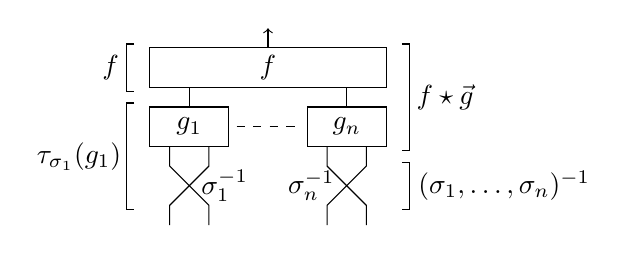
\begin{tikzpicture}
\draw (0,0) -- (3,0) -- (3,-0.5) -- (0,-0.5) -- cycle;
\node at (1.5,-0.25) {$f$};
\draw[->] (1.5,0) -- (1.5,0.25);
\draw (0.5,-0.5) -- (0.5,-.75);
\draw (0,-.75) -- (1,-.75) -- (1,-1.25) -- (0,-1.25) -- cycle;
\node at (0.5,-1) {$g_1$};
\draw (0.25,-1.25) -- (0.25,-1.5) -- (0.75,-2) -- (0.75,-2.25);
\draw (0.75,-1.25) -- (0.75,-1.5) -- (0.25,-2) -- (0.25,-2.25);
\node at (0.95,-1.75) {$\tiny \sigma_1^{-1}$};
\draw[dashed] (1.1,-1) -- (1.9,-1);
\draw (2.5,-0.5) -- (2.5,-.75);
\draw (2,-.75) -- (3,-.75) -- (3,-1.25) -- (2,-1.25) -- cycle;
\node at (2.5,-1) {$g_n$};
\draw (2.25,-1.25) -- (2.25,-1.5) -- (2.75,-2) -- (2.75,-2.25);
\draw (2.75,-1.25) -- (2.75,-1.5) -- (2.25,-2) -- (2.25,-2.25);
\node at (2.05,-1.75) {$\tiny \sigma_n^{-1}$};
\draw (-0.2,0.05) -- (-0.3,0.05) -- (-0.3,-0.55) -- (-0.2,-0.55);
\draw (-0.2,-0.7) -- (-0.3,-0.7) -- (-0.3,-2.05) -- (-0.2,-2.05);
\draw (3.2,0.05) -- (3.3,0.05) -- (3.3,-1.3) -- (3.2,-1.3);
\draw (3.2,-1.45) -- (3.3,-1.45) -- (3.3,-2.05) -- (3.2,-2.05);
\node at (-0.5,-0.25) {$f$};
\node at (-0.9,-1.375) {$\tau_{\sigma_1}(g_1)$};
\node at (3.75,-.625) {$f \star \vec{g}$};
\node at (4.5,-1.75) {$(\sigma_1,\ldots,\sigma_n)^{-1}$};
\end{tikzpicture}

\end{document}